\documentclass[12pt]{article}
\usepackage[a3paper,landscape,left=1.3cm,right=1.3cm,top=1.4cm,bottom=1.4cm,columnsep=0.9cm,headheight=18pt,footskip=15pt]{geometry}
\usepackage{xeCJK}
\setCJKmainfont{SimSun}
\setCJKsansfont{Microsoft YaHei}
\setCJKmonofont{FangSong}
\usepackage{amsmath,amssymb}
\usepackage{tikz}
\usetikzlibrary{angles,quotes,calc,intersections,arrows.meta}
\usepackage{fancyhdr}
\usepackage{enumitem}
\usepackage{multicol}
\usepackage{tabularx}
\usepackage{array}
\usepackage{xcolor}
\usepackage{tcolorbox}
\usepackage{lastpage}

\newif\ifanswers
\ifdefined\withanswers
  \answerstrue
\else
  \answersfalse
\fi

\setlength{\parindent}{0pt}
\setlength{\parskip}{0.2em}
\setlength{\columnseprule}{0.25pt}
\setlength{\columnsep}{0.9cm}
\renewcommand{\arraystretch}{1.25}
\raggedcolumns

\pagestyle{fancy}
\fancyhf{}
\fancyhead[L]{育才中学 2025--2026 学年度第一学期}
\fancyhead[C]{九年级数学期末考试试卷}
\fancyhead[R]{考试时间:120分钟\quad 满分:120分}
\fancyfoot[C]{第\thepage 页 / 共\pageref{LastPage}页}
\renewcommand{\headrulewidth}{0.4pt}
\renewcommand{\footrulewidth}{0pt}

\tcbset{
  colback=white,
  colframe=gray!65,
  boxrule=0.45pt,
  arc=1mm,
  left=1mm,right=1mm,top=1mm,bottom=1mm
}
\newtcolorbox{answerbox}[1][3.2cm]{height=#1}

\newcommand{\analysis}[1]{%
  \ifanswers
    {\par\small\color{blue!70!black}\textbf{解析:}#1\par\normalsize}
  \fi
}

\newcommand{\parttitle}[1]{\vspace{0.4em}\textbf{\large #1}\par\vspace{0.3em}}

\begin{document}

\begin{center}
  {\Large\bfseries 九年级数学期末考试试卷}
\end{center}

\vspace{-0.4em}
\begin{tabularx}{\textwidth}{|>{\raggedright\arraybackslash}X|>{\raggedright\arraybackslash}X|>{\raggedright\arraybackslash}X|>{\raggedright\arraybackslash}X|}
\hline
姓名:\underline{\hspace{3.2cm}} &
班级:\underline{\hspace{2.5cm}} &
学号:\underline{\hspace{2.5cm}} &
座位号:\underline{\hspace{2.2cm}} \\
\hline
\multicolumn{4}{|l|}{注意事项:1. 本卷共三大题,满分 120 分;2. 解答题需写出必要步骤;3. 请在答题区域内作答。} \\
\hline
\end{tabularx}

\vspace{0.5em}
\begin{multicols}{2}

\parttitle{一、选择题(本大题共10小题,每小题3分,共30分)}
\begin{enumerate}[leftmargin=1.8em,label=\textbf{\arabic*.},itemsep=0.9em]
  \item 若关于 $x$ 的方程 $x^2-(m+1)x+m=0$ 有两个相等实数根,则 $m$ 的值为(\hspace{2em})\\
  A. $-1$\hfill B. $0$\hfill C. $1$\hfill D. $2$\\
  答案:\underline{\hspace{2.4cm}}

  \item 过点 $(1,2)$ 且与直线 $y=-3x+5$ 平行的直线解析式为(\hspace{2em})\\
  A. $y=-3x+2$\hfill B. $y=-3x+5$\hfill C. $y=3x-1$\hfill D. $y=3x+5$\\
  答案:\underline{\hspace{2.4cm}}

  \item 不等式组 $\begin{cases}2x-1>3\\ x+4\le 7\end{cases}$ 的解集为(\hspace{2em})\\
  A. $x>2$\hfill B. $x\le 3$\hfill C. $2<x\le3$\hfill D. $x\ge 3$\\
  答案:\underline{\hspace{2.4cm}}

  \item 抛物线 $y=(x-2)^2-3$ 的顶点坐标是(\hspace{2em})\\
  A. $(2,-3)$\hfill B. $(-2,-3)$\hfill C. $(2,3)$\hfill D. $(-2,3)$\\
  答案:\underline{\hspace{2.4cm}}

  \item 在 $\triangle ABC$ 中,$\angle C=90^\circ$,$\tan A=\frac{3}{4}$,则 $\sin A$ 等于(\hspace{2em})\\
  A. $\frac{3}{5}$\hfill B. $\frac{4}{5}$\hfill C. $\frac{5}{3}$\hfill D. $\frac{4}{3}$\\
  答案:\underline{\hspace{2.4cm}}

  \item 某小组 5 次测验成绩为 $86,90,90,92,97$,则这组数据的中位数为(\hspace{2em})\\
  A. $90$\hfill B. $91$\hfill C. $92$\hfill D. $97$\\
  答案:\underline{\hspace{2.4cm}}

  \item 已知点 $P(2,3)$ 在反比例函数 $y=\frac{k}{x}$ 图象上,则该函数图象一定经过(\hspace{2em})\\
  A. $(1,3)$\hfill B. $(3,2)$\hfill C. $(-2,-3)$\hfill D. $(-3,2)$\\
  答案:\underline{\hspace{2.4cm}}

  \item 若两个相似三角形的周长比为 $2:3$,则它们的面积比为(\hspace{2em})\\
  A. $2:3$\hfill B. $3:2$\hfill C. $4:9$\hfill D. $9:4$\\
  答案:\underline{\hspace{2.4cm}}

  \item 袋中有红球 3 个、白球 2 个、蓝球 1 个,随机摸出 1 个球,摸到白球的概率为(\hspace{2em})\\
  A. $\frac{1}{6}$\hfill B. $\frac{1}{3}$\hfill C. $\frac{1}{2}$\hfill D. $\frac{2}{3}$\\
  答案:\underline{\hspace{2.4cm}}

  \item 二次函数 $y=x^2-4x+c$ 的最小值是 $-1$,则 $c$ 的值为(\hspace{2em})\\
  A. $2$\hfill B. $3$\hfill C. $4$\hfill D. $5$\\
  答案:\underline{\hspace{2.4cm}}
\end{enumerate}

\parttitle{二、填空题(本大题共6小题,每小题3分,共18分)}
\begin{enumerate}[leftmargin=1.8em,label=\textbf{\arabic*.},start=11,itemsep=1.0em]
  \item 若 $a,b$ 是方程 $x^2-4x-1=0$ 的两个根,则 $a^2+b^2=$\underline{\hspace{3cm}}。\\[0.6em]
  \item 抛物线 $y=-x^2+2x+3$ 与 $x$ 轴两交点间距离为\underline{\hspace{3cm}}。\\[0.6em]
  \item 方程 $(x-1)^2+2=2x+1$ 的较小根为\underline{\hspace{3cm}}。\\[0.6em]
  \item 在圆中,若圆心角为 $120^\circ$,对应弧长为 $4\pi$,则该圆半径为\underline{\hspace{3cm}}。\\[0.6em]
  \item 一组数据 $2,3,3,4,5,a$ 的平均数是 $4$,则 $a=$\underline{\hspace{3cm}}。\\[0.6em]
  \item 若点 $M(2,m)$ 与点 $N(-4,m)$ 在函数 $y=(k-1)x+3$ 图象上,则 $k=$\underline{\hspace{3cm}}。\\[0.6em]
\end{enumerate}

\parttitle{三、解答题(本大题共8小题,共72分)}

\textbf{17.(8分)}计算与解不等式:\\
(1)解方程:$\dfrac{x-1}{2}+\dfrac{x+3}{3}=4$;\\
(2)解不等式组:$\begin{cases}3x-5\le 7\\ 2x+1>5\end{cases}$。\\
\begin{answerbox}[4.8cm]\end{answerbox}
\analysis{(1)去分母得 $3(x-1)+2(x+3)=24$,解得 $x=\frac{21}{5}$。 (2)由两式得 $x\le4,\ x>2$,故解集为 $2<x\le4$。}

\textbf{18.(8分)}已知一次函数图象经过点 $A(-1,2)$、$B(3,-4)$。\\
(1)求该一次函数解析式;\\
(2)设该函数图象与 $x$ 轴交于点 $C$,求 $\triangle AOC$ 的面积($O$ 为原点)。\\
\begin{answerbox}[5.2cm]\end{answerbox}
\analysis{设函数为 $y=kx+b$,由两点坐标得 $k=-\frac{3}{2},b=\frac{1}{2}$,故 $y=-\frac{3}{2}x+\frac{1}{2}$。令 $y=0$,得 $C\left(\frac13,0\right)$。由坐标法,$S_{\triangle AOC}=\frac12\left|x_Ay_C-x_Cy_A\right|=\frac13$。}

\textbf{19.(8分)}如图,在等腰三角形 $ABC$ 中,$AB=AC$,点 $D$ 为 $BC$ 中点。过点 $D$ 分别作 $DE\perp AB$ 于点 $E$,$DF\perp AC$ 于点 $F$。\\
\begin{center}
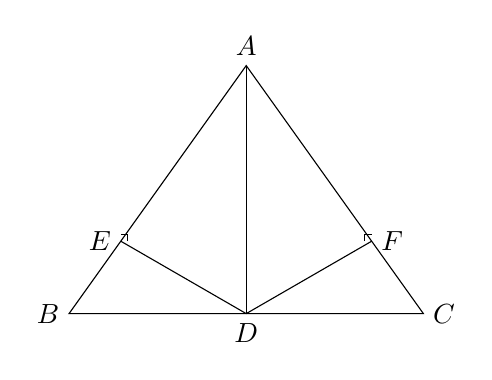
\begin{tikzpicture}[scale=0.75]
  \coordinate (B) at (0,0);
  \coordinate (C) at (6,0);
  \coordinate (A) at (3,4.2);
  \coordinate (D) at (3,0);
  \path[name path=AB] (A)--(B);
  \path[name path=AC] (A)--(C);
  \path[name path=perpDAB] (D)--++(150:3.5);
  \path[name path=perpDAC] (D)--++(30:3.5);
  \path[name intersections={of=AB and perpDAB,by=E}];
  \path[name intersections={of=AC and perpDAC,by=F}];
  \draw (A)--(B)--(C)--cycle;
  \draw (D)--(E) (D)--(F);
  \draw (A)--(D);
  \draw ($(E)+(0.12,0)$)--++(0,0.12)--++(-0.12,0);
  \draw ($(F)+(-0.12,0)$)--++(0,0.12)--++(0.12,0);
  \node[above] at (A) {$A$};
  \node[left] at (B) {$B$};
  \node[right] at (C) {$C$};
  \node[below] at (D) {$D$};
  \node[left] at (E) {$E$};
  \node[right] at (F) {$F$};
\end{tikzpicture}
\end{center}
(1)求证:$DE=DF$;\\
(2)若 $\angle BAC=40^\circ$,求 $\angle EDF$ 的度数。\\
\begin{answerbox}[5.8cm]\end{answerbox}
\analysis{由 $AB=AC$ 且 $D$ 为 $BC$ 中点,得 $AD$ 为 $\angle A$ 平分线。点到角两边距离相等,故 $DE=DF$。又 $DE\perp AB,\ DF\perp AC$,两垂线夹角等于对应边夹角,故 $\angle EDF=\angle BAC=40^\circ$。}

\textbf{20.(8分)}某班 10 名同学一次“立定跳远提升量(cm)”数据为:\\
$6,\ 8,\ 7,\ 10,\ 9,\ 8,\ 7,\ 11,\ 9,\ 15$。\\
(1)求这组数据的平均数与中位数;\\
(2)从这 10 名同学中随机抽取 2 名,求“至少有 1 名同学提升量不低于 10cm”的概率。\\
\begin{answerbox}[6.2cm]\end{answerbox}
\analysis{(1)平均数 $\frac{90}{10}=9$,排序后中位数为第5、6个数平均,即 $\frac{8+9}{2}=8.5$。 (2)不低于10cm有3人,低于10cm有7人。所求概率 $=1-\frac{\binom72}{\binom{10}2}=1-\frac{21}{45}=\frac{8}{15}$。}

\textbf{21.(10分)}如图,在矩形 $ABCD$ 中,$AB=8,\ BC=6$。点 $E$ 在边 $AB$ 上,且 $AE=2$,过点 $E$ 作 $EF\parallel BC$,交对角线 $AC$ 于点 $F$。\\
\begin{center}
\begin{tikzpicture}[scale=0.72]
  \coordinate (A) at (0,0);
  \coordinate (B) at (8,0);
  \coordinate (C) at (8,6);
  \coordinate (D) at (0,6);
  \coordinate (E) at (2,0);
  \path[name path=AC] (A)--(C);
  \path[name path=Ev] (E)--++(0,7);
  \path[name intersections={of=AC and Ev,by=F}];
  \draw (A)--(B)--(C)--(D)--cycle;
  \draw (A)--(C);
  \draw (E)--(F);
  \draw (D)--(F);
  \node[below left] at (A) {$A$};
  \node[below right] at (B) {$B$};
  \node[above right] at (C) {$C$};
  \node[above left] at (D) {$D$};
  \node[below] at (E) {$E$};
  \node[right] at (F) {$F$};
\end{tikzpicture}
\end{center}
(1)求证:$\triangle AEF \sim \triangle ABC$,并求 $AF$ 的长;\\
(2)求 $DF$ 的长。\\
\begin{answerbox}[8.0cm]\end{answerbox}
\analysis{因 $EF\parallel BC$,得 $\angle AEF=\angle ABC,\ \angle AFE=\angle ACB$,故两三角形相似。$\frac{AE}{AB}=\frac{AF}{AC}=\frac{2}{8}=\frac14$。又 $AC=\sqrt{8^2+6^2}=10$,故 $AF=2.5$。取坐标法得 $F(2,1.5),\ D(0,6)$,故 $DF=\sqrt{(2-0)^2+(1.5-6)^2}=\frac{\sqrt{97}}{2}$。}

\columnbreak

\textbf{22.(10分)}已知抛物线 $y=ax^2+bx+c$ 经过点 $A(-1,0)$、$B(3,0)$、$C(0,3)$。\\
(1)求该抛物线解析式;\\
(2)求顶点坐标;\\
(3)若点 $M$ 在该抛物线上且 $x_M>3$,过 $M$ 作 $x$ 轴垂线交 $x$ 轴于 $N$。当 $\triangle BMN$ 的面积为 $12$ 时,求点 $M$ 的坐标。\\
\begin{answerbox}[9.2cm]\end{answerbox}
\analysis{由两根得 $y=a(x+1)(x-3)$,代入 $C(0,3)$ 得 $a=-1$,故 $y=-x^2+2x+3$。顶点 $P(1,4)$。设 $M(t,-t^2+2t+3)$,$t>3$,则 $N(t,0)$。有 $BN=t-3,\ MN=t^2-2t-3=(t-3)(t+1)$。由 $\frac12\cdot BN\cdot MN=12$ 得 $(t-3)^2(t+1)=24$,解得 $t=5$。故 $M(5,-12)$。}

\textbf{23.(10分,压轴)}在平面直角坐标系中,设点 $P(t,0)$($t<1$),过点 $P$ 作斜率为 $1$ 的直线 $l:y=x-t$,与抛物线 $C:y=x^2-4x+3$ 交于 $M,N$ 两点($M$ 在 $N$ 左侧)。\\
(1)当 $t=-1$ 时,求点 $M,N$ 的坐标;\\
(2)求线段 $MN$ 的长度(用 $t$ 表示);\\
(3)设 $O$ 为原点,若 $\triangle OMN$ 的面积为 $\dfrac{15}{2}$,求 $t$ 的值。\\
\begin{answerbox}[11.5cm]\end{answerbox}
\analysis{联立得 $x^2-5x+(3+t)=0$,设两根为 $x_1<x_2$。 (1)$t=-1$ 时,$x_{1,2}=\frac{5\pm\sqrt{17}}2$,故 $M\!\left(\frac{5-\sqrt{17}}2,\frac{7-\sqrt{17}}2\right)$,$N\!\left(\frac{5+\sqrt{17}}2,\frac{7+\sqrt{17}}2\right)$。 (2)$|x_2-x_1|=\sqrt{13-4t}$,又直线斜率为1,故 $MN=\sqrt2\,|x_2-x_1|=\sqrt{2(13-4t)}$。 (3)$S_{\triangle OMN}=\frac12|x_1y_2-x_2y_1|=\frac{|t|}{2}|x_2-x_1|=\frac{|t|}{2}\sqrt{13-4t}$。令其等于 $\frac{15}{2}$,得 $|t|\sqrt{13-4t}=15$。由 $t<1$ 可判定 $t<0$,解得 $t=-3$。}

\textbf{24.(10分,压轴)}如图,在圆 $\omega$ 中,$AB$ 为直径,点 $C$ 在圆上($C\neq A,B$),过点 $C$ 的切线与直线 $AB$ 交于点 $D$($A$ 在 $B,D$ 之间)。连接 $AC,BC$。\\
\begin{center}
\begin{tikzpicture}[scale=0.78]
  \coordinate (A) at (0,0);
  \coordinate (B) at (8,0);
  \coordinate (O) at (4,0);
  \coordinate (C) at (2.5,3.708);
  \path[name path=ABline] (-2,0)--(12,0);
  \path[name path=tangent] (C)--++(-2.4,1.0);
  \path[name intersections={of=ABline and tangent,by=D}];
  \coordinate (M) at ($(C)!0.55!(D)$);
  \path[name path=AC] (A)--(C);
  \path[name path=MNline] (M)--++(8,0);
  \path[name intersections={of=AC and MNline,by=N}];
  \draw (O) circle (4);
  \draw (-1.5,0)--(10.5,0);
  \draw (A)--(C)--(B);
  \draw (C)--(D);
  \draw (M)--(N);
  \fill (M) circle (1.2pt) (N) circle (1.2pt);
  \node[below] at (A) {$A$};
  \node[below] at (B) {$B$};
  \node[below] at (O) {$O$};
  \node[above] at (C) {$C$};
  \node[below] at (D) {$D$};
  \node[above left] at (M) {$M$};
  \node[above left] at (N) {$N$};
\end{tikzpicture}
\end{center}
(1)证明:$\angle ACD=\angle CBA$,并由此证明 $DC^2=DA\cdot DB$;\\
(2)若 $AB=10,\ DC=12$,求 $AD$ 的长;\\
(3)点 $M$ 在线段 $CD$ 上,过 $M$ 作 $MN\parallel AB$ 交 $AC$ 于点 $N$。探究 $\frac{CN}{CA}$ 与 $\frac{CM}{CD}$ 的关系,并说明理由。\\
\begin{answerbox}[14.2cm]\end{answerbox}
\analysis{(1)切线与弦所夹角等于所对圆周角,故 $\angle ACD=\angle CBA$。进一步由相似关系得到切割线定理 $DC^2=DA\cdot DB$。 (2)设 $AD=x$,则 $DB=x+10$,由 $x(x+10)=144$ 得 $x=8$(舍负根),故 $AD=8$。 (3)因 $MN\parallel AB$,且 $AB$ 与 $AD$ 共线,在 $\triangle CDA$ 中有 $\triangle CMN\sim\triangle CDA$,故 $\frac{CN}{CA}=\frac{CM}{CD}$。}

\ifanswers
\vspace{0.8em}
\textbf{选择题答案:}1.C\ 2.B\ 3.C\ 4.A\ 5.A\ 6.A\ 7.C\ 8.C\ 9.B\ 10.B\\
\textbf{填空题答案:}11.18\ 12.4\ 13.$2-\sqrt2$\ 14.6\ 15.7\ 16.1
\fi

\end{multicols}
\end{document}
